\chapter{Simulation}
\label{ch:simulation}

Monte Carlo simulation (MC) refers to the practice
of estimating the probability distribution of the outcomes
of a complex and non-deterministic chain of events
by running a (pseudo-random) simulation of the process multiple times
and recording the distribution of the simulated outcomes.
MC is commonly used to estimate detection efficiencies,
a detector's energy response,
and other quantities that have a highly nontrivial dependence
on basic geometric and kinematic quantities.

A distinction is often made between a ``full Monte Carlo''
and a ``toy Monte Carlo.''
In a full MC, each particle is propagated through a series of small time steps,
with various probabilities to interact, decay, deposit energy, and/or be detected,
depending on the material being traversed.
As the name suggests, toy MCs adopt simplifications from the full approach,
and these simplifications can vary widely.
One prototypical example is to use the average $\nicefrac{dE}{dx}$
and a particle's propagation distance
(perhaps determined by drawing from an exponential distribution
based on the decay time and velocity)
to determine the amount of energy deposited by a particle
before it decays.
The simplifications made to toy MCs usually limit their validity
to highly specific scenarios.

Three separate toy MC simulations were used in this analysis
to simulate individual IBD events (\cref{sec:thu_toymc}),
Daya Bay reconstructed-data files (\cref{sec:toymc}),
and entire experiments' worth of data (\cref{sec:lbnl_toymc}).

\section{Individual IBD event simulation}
\label{sec:thu_toymc}

The Individual Event Simulation (IES) was designed
to study detection efficiencies and the detector energy response \cite{nh2016technote}.
This simulation was composed of a full, particle-level Monte Carlo simulation
and a toy detector response model.
Each event began as a \nuebar{} of a given energy interacting via IBD
with an atom in a given region of the Daya Bay AD
(GdLS, LS or acrylic).
The interaction products ($e^+$ and $n$),
were simulated using a full MC implemented using the GEANT4 library \cite{geant4}.
The full simulation included
the positron's energy depositions into the scintillator
and its annihilation,
the neutron's thermalization, scattering, and capture on a nucleus (or escape),
and the resulting $\gamma$-rays' propagation and interactions.
The resulting electrons and positrons from the $\gamma$-ray interactions
were also simulated.
During propagation, an electron could
``deposit'' energy in the liquid scintillator,
escape from the scintillating volume,
or scatter and create another energetic electron.
The total amount of deposited energy was saved as $E_{\text{dep}}$.

To obtain a final simulated reconstructed energy,
a parametrized nonlinearity model and resolution were used
rather than implementing the effects in a full MC.
The scintillator and electronics nonlinearities were applied
to the deposited energy $E_{\text{dep}}$
(see \cref{subsec:abs_energyscale}).
The energy resolution (\cref{subsec:resolution}) used in the MC
was modified to reflect
the absence of detector non-uniformity in the simulation
by setting the $a$ parameter to 0 (cf.\ \cref{eq:energy_resolution}):
\begin{equation}
    \frac{\sigma_E}{E} = \sqrt{0 + \frac{b^2}{E} + \frac{c^2}{E^2}}.
\end{equation}

The IES was used to generate a data set
where the incident \nuebar{} spectrum
matched the predicted unoscillated reactor \nuebar{} spectrum.
The distributions of simulated prompt and delayed reconstructed energies,
shown in \cref{fig:prompt_eff_mc},
could be used as estimates of the actual distributions.
In other analyses (e.g.\ \cite{nh2016}), the MC estimates
for absolute efficiencies of the prompt and delayed energy cuts
were computed from this simulation.
In this analysis, the absolute efficiencies were not used.
However, the IES was used to estimate other quantities.

\begin{figure}
    \centering
    \includegraphics[width=0.49\textwidth]{%
        ch_event_selection/prompt_energy_mc%
    }
    \includegraphics[width=0.49\textwidth]{%
        ch_event_selection/delayed_energy_mc%
    }
    \caption[Simulated prompt and delayed spectra]{Spectrum of reconstructed energy for simulated IBD prompt (left)
        and delayed (right) events
        in the Monte Carlo study used to compute the absolute efficiencies
        of the prompt- and delayed- energy cuts.
        The prompt spectrum is also used to compute the
        AD-uncorrelated uncertainty of the prompt-energy cut.
    }
    \label{fig:prompt_eff_mc}
\end{figure}

\subsubsection{Study of prompt energy cut efficiency}

The prompt-energy cut efficiency for each AD depended on
the oscillation parameters due to the energy dependence of \nuebar{} oscillation
(see \cref{subsec:prompt_energy}).
This correction was computed at a given point in parameter space
(value of \thetaot{}, $\Delta m^2_{32}$, and AD-reactor pair)
by creating a histogram of reconstructed prompt energy
where each entry was weighted by the oscillation probabilty
at the ``true'' \nuebar{} energy saved by the simulation.
The resulting efficiency was compared
with the nominal efficiency assuming no oscillation.
The relative difference was applied as a correction
during the near-far projection procedure in \cref{subsec:flux_fraction}.

\subsubsection{Study of relative energy scale}

The prompt-energy spectrum and cut efficiency
both depended on the relative energy scale between ADs
(see \cref{subsec:rel_energyscale}).
A shift in the energy scale was modeled by
creating a histogram of reconstructed prompt energy,
but where the value of the energy was scaled
by the uncertainty of the relative energy scale, \SI{\pm0.5}{\percent}.
The resulting change to the prompt-energy cut efficiency, \SI{\pm0.1}{\percent},
was the AD-uncorrelated uncertainty for that efficiency.
Shifting the energy scale also changed the shape of the spectrum,
which was quantified by comparing the change in number of events
in each bin of the histogram with and without the re-scaled energy values.
The oscillation dependence of the spectral shape was also accounted for.

For a particular bin $b$ of reconstructed energy in AD $i$,
the relative energy scale correction $a_{\text{relE},i}^{(b)}$
was defined as the difference in bin content with and without
the relative energy scale shift of \SI{\pm0.5}{\percent},
divided by the bin content without the shift:
\begin{equation}
    a_{\text{relE},i}^{\pm,(b)}(\thetaot, \Delta m^2_{32}) =
    \frac{N^\pm(\thetaot, \Delta m^2_{32}) - N^0(\thetaot, \Delta m^2_{32})}%
    {N^0(\thetaot, \Delta m^2_{32})},
\end{equation}
where the $+$ refers to scaling the energy by \SI[retain-explicit-plus]{+0.5}{\percent}
and the $-$ refers to scaling by \SI{-0.5}{\percent}.
During the fit procedure to extract \thetaot{} in \cref{ch:analysis}, the impact of this correction
was controlled by a nuisance parameter.
The fitter automatically switched between the $+$ and $-$ values
depending on the sign of the nuisance parameter.

This correction was intentionally not normalized;
the consistent application of $a_{\text{relE},i}^{\pm,(b)}$ to all bins
could change the total number of events.
The impact of the change in total number of events
was equivalent to the previously-mentioned change
to the prompt-energy cut efficiency induced by the relative energy scale shift.
To avoid double-counting the change in number of events
due to a shift in relative energy scale,
the prompt-energy cut efficiency was omitted
from the fit model and from the constraint
on the nuisance parameter representing the overall detection efficiency uncertainty.

\section{Data file simulation}
\label{sec:toymc}

The Daya Bay event selection process (\cref{ch:event_selection})
depended on more than just the properties of each AD event in isolation;
there were anti-coincidence requirements such as the muon veto,
and of course double-coincidence requirements to select IBDs.
Additionally, the basis for the determination of the accidental background rate
relied heavily on the accurate extraction of
the rate of uncorrelated ``single'' events.
Both the event selection and the accidentals characterization
relied on a simple model of the data stream,
with only three distinct event types:
muon events, uncorrelated single events,
and correlated pairs comprising IBD events.
The Reconstructed-Data File Simulation (RDFS)
produced simulated data files in the same format
as the output of the calibration and reconstruction procedure
(``production,'' described in \cref{sec:daq}).
This simulation was used
to study the impact of the assumptions in the data stream model
and to validate the implementation of
the event selection and accidentals characterization
in software.

The RDFS received as input
a specification for the rates of various event types,
representing IBDs, uncorrelated events, muons, etc.,
and a total ``runtime'' representing the amount of AD livetime to simulate.
The configuration could be varied to, for example,
increase the rate of single events
or decrease the capture time delay between prompt and delayed IBD signals.
and the effect of that change could be studied.
To produce a data stream,
first, timestamps were generated for each event
based on the rates for each event type and the total livetime.
Simulated energy and position values were then generated for each event.
Vast simplifications were employed to allow for
extremely fast event generation,
and no attempt was made at creating
physically-realistic distributions for
reconstructed energy or position.
Instead, these distributions were chosen to make analysis
of the selection cuts more convenient.
This was an acceptable compromise since the purpose of the simulation
was to validate properties of the data model,
rather than the traditional goal of estimating specific quantities
which are difficult or impossible to measure using real data.

Simulated events were saved to disk in the same ROOT file data format
used by the Daya Bay data production.
An additional ROOT TTree structure containing the ``truth information''
for each event was included in the output data file.
For this simulation, the truth information for an event consisted simply of
the event type.
A flowchart describing the steps in the simulation
is provided in \cref{fig:my_toymc_flowchart}.
The characteristics associated with the different event types
are described below.

\begin{figure}
    \centering
    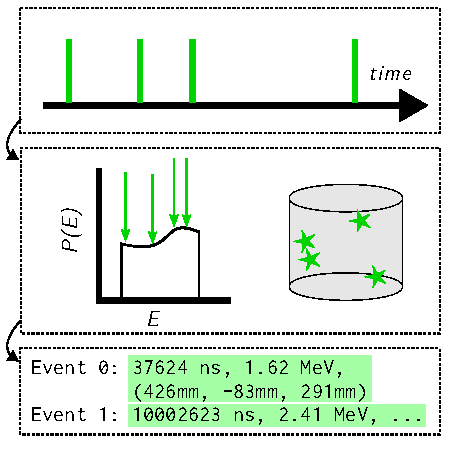
\includegraphics[width=0.49\textwidth]{ch_simulation/singles_flow}
    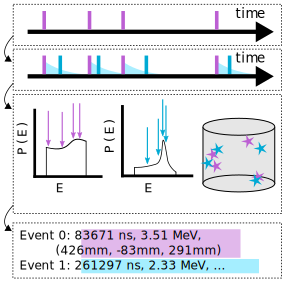
\includegraphics[width=0.49\textwidth]{ch_simulation/correlated_flow}
    \caption[Data stream simulation diagram]{
        The data stream simulation steps
        for Single events (left) and Correlated events (right).
        The steps are event count and timestamps (top),
        energy and position (middle), and serialization (bottom).
        Different colors represent different event types:
        green, violet and blue represent Single,
        prompt Correlated and delayed Correlated,
        respectively.
        The highlight colors in the serialization phase
        represent the ``truth'' information stored separately.
    }
    \label{fig:my_toymc_flowchart}
\end{figure}


The RDFS was based on a core set of event types:
Single, Correlated, and Muon.
Additional event types such as Flasher were added to support specific studies
(see \cref{subsec:toymc_flashers}).
The simulation's configuration allowed for customization of the event rate
for each different event type,
and also for multiple variants of the event type.
For example, one type of Correlated event could be configured to represent nH IBDs,
and a second type could be configured to represent nGd IBDs
with a shorter coincidence time, higher delayed energy,
and with the delayed event's position limited to the GdLS (IAV) region of the AD.

\subsection{Types of generated events}

\subsubsection{Single events}

Single events represented uncorrelated signals,
which in Daya Bay were primarily caused by natural radioactive decays in the AD
(\cref{subsec:singles}).
In the simulation, Single events were assigned timestamps
drawn uniformly at random between the runtime limits given in the configuration,
representing their uncorrelated nature.
The event energies were also drawn uniformly at random
between \SIlist{1;3.5}{\MeV},
and the positions were randomly assigned
within the scintillating volume.
(The energy and position distributions can both be customized through plug-ins
but were left at their defaults for the studies described here.)

\subsubsection{Correlated events}

Correlated events represented pairs of signals
with a common physical origin, both in position and in time.
IBDs and correlated backgrounds (\cref{sec:correlated_bg})
satisfied these criteria and could be modeled by the Correlated event type.
To create the time correlation between prompt and delayed events,
modeled as an exponential distribution,
the simulation first determined the timestamp for a prompt event at random.
Then the coincidence time delay between prompt and delayed events was generated
from an exponential distribution
whose time constant was specified in the simulation configuration.
The prompt and delayed energies were determined independently at random
using distributions specified by the simulation configuration.
The position of the prompt event was chosen at random
within the GdLS or LS volumes (again, as specified by the configuration),
and the delayed position was chosen to be correlated with the prompt position.
Since exact modeling of the position correlations was not crucial for the studies
performed with the RDFS,
a simple exponential distribution was used to determine the displacement
in each direction ($x,y,$ and $z$) for these Correlated events.
In the recorded truth information,
prompt and delayed events are assigned separate labels.

\subsubsection{Muon events}

Muon events represented signals created by muons traversing
the water pools and ADs (\cref{sec:muonveto}).
For simplicity, each muon was assumed to create a signal
in the inner water pool with a probability of \SI{100}{\percent}.
The rates and energies were chosen to approximately model
the true distributions and rates of muon signals in the near halls (EH1 and EH2).
A portion of the muon signals, \SI{19.95}{\percent},
were assumed to traverse the AD, depositing an energy chosen at random between
\SIlist{20;2000}{\MeV}.
A smaller subset of the muon signals, \SI{0.05}{\percent},
were simulated as showering muons and deposited an energy chosen at random between
\SIlist{2500;5000}{\MeV}.
The time delay between WP and AD muons was assigned to be \SI{50}{\ns},
chosen since in real data there was a nonzero time offset between WP and AD muons;
however, the precise distribution of time offsets between WP and AD muon readout signals
was not a critical feature of the event selection.
All of the choices of energies and rates were approximations
designed to capture the general behavior of muons at Daya Bay
without adding excessive complexity to the simulation.

\subsection{Study of uncorrelated-event rate}
\label{subsec:sim_singles}

The procedure for determining the uncorrelated-event rate
is described in \cref{subsec:singles}.
This process, both the abstract algorithm and the actual software implementation,
was validated using simulated datasets.
The RDFS was configured to generate Single (uncorrelated) events
with a rate of \SI{20}{\Hz}
in data files also containing Muon and Correlated events
representing both nH and nGd IBDs.
The full configuration is listed in \cref{tab:toymc_singles_config}.
100 simulated data files were generated,
each containing 1000 minutes' worth of data.
The data files were processed using the event selection software
and an empirical rate for uncorrelated events was extracted
for each of the 100 files.
The distribution of measured uncorrelated event rates
is shown in \cref{fig:toymc_singles_dist}.
The mean rate over all 100 data sets
was \SI{19.9966+-0.0022}{\Hz},
which is a bias of \SI{0.017}{\percent} or 2 standard deviations.
This bias was considered acceptable
since the accidentals rate uncertainty
for the actual data set was approximately \SI{0.077}{\percent}.
Thus the simulation was able to confirm that
the event selection software could successfully extract
the uncorrelated-event rate with high precision and tolerable bias.

\begin{table}[ht]
    \centering
    \begin{tabular}[t]{lSlS}
        \toprule
        Event type & {Rate [\si{\Hz}]} & Energy [\si{\MeV}] & {Coincidence time [\si{\us}]}\\
        \midrule
        Single & 20. & $[\num{1.5}, \num{3}]$ & {-}\\
        Correlated prompt (nH) & 0.005 & [0.7, 4] & {-} \\
        Correlated delayed (nH) & {-} & [1.9, 2.3] & 150. \\
        Correlated prompt (nGd) & 0.0067 & [0.7, 4] & {-} \\
        Correlated delayed (nGd) & {-} & [7, 9] & 28. \\
        Water Pool Muon & 200. & - & {-} \\
        AD Muon & 39.9 & [\num{20}, \num{2000}] & {-}\\
        Showering Muon & 0.1 & [\num{2500}, \num{5000}] & {-}\\
        \bottomrule
    \end{tabular}
    \caption[Uncorrelated event simulation inputs]{
        Simulation configuration inputs for the uncorrelated-event rate study.
        The rates, energies and coincidence times were simplified
        to allow for faster simulation,
        and no results based on the specific distributions of these quantities
        were used in the final analysis.
    }
    \label{tab:toymc_singles_config}
\end{table}

\begin{figure}
    \centering
    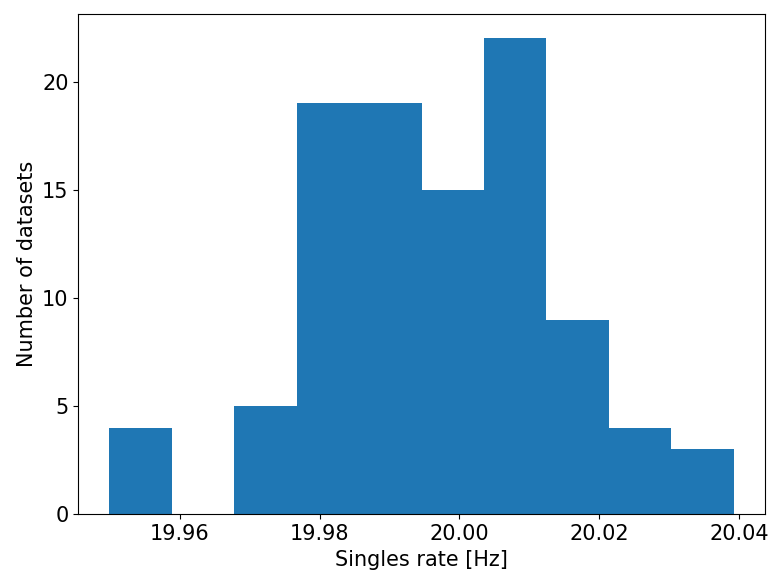
\includegraphics[width=0.7\textwidth]{ch_simulation/singles_rate_unbiased_dist}
    \caption[Extracted simulated uncorrelated event rates]{
        Distribution of uncorrelated event rates over 100 simulated data sets.
        The simulation configuration (``truth'') specified a rate of \SI{20}{\Hz}.
        Each data set consists of a single 1000-minute data file.
    }
    \label{fig:toymc_singles_dist}
\end{figure}

\subsection{Study of residual flashers}
\label{subsec:toymc_flashers}

Light emission by PMTs caused a background of single events
known as flashers \cref{sec:flashers}.
The vast majority of flasher events were rejected using an event-by-event veto,
and the remaining flashers were assumed to be accounted for
by the treatment of the accidental background (\cref{sec:acc}).
Certain PMTs were observed to flash with a frequency
of approximately \SI{0.1}{\Hz},
but with the restriction that
the same PMT never flashed twice within $\lesssim$\SI{0.7}{\s}
(see \cref{fig:flasher_anticorr}).
This pattern violated the assumption in the accidental background analysis
that all single events were uncorrelated and governed by Poisson statistics.
A Flasher event type was added to the RDFS to test the impact of this deviation.

The Flasher event type had a fixed energy and position.
Generated Flasher events were assigned fixed, deterministic timestamps \SI{1}{\s} apart
to simulate a maximally-anticorrelated process with no possible time coincidences.
A data sample was generated with only Single events and Flasher events,
and was treated as if the Flasher events passed the flasher veto criteria.
The Single events had the same configuration as in \cref{tab:toymc_singles_config},
and the Flasher events were assigned a fixed energy of \SI{2.7}{\MeV}.
The accidental background analysis was performed on this data sample (\cref{sec:acc});
after subtracting the accidental background,
the expectation was that 0 correlated events should remain.
\Cref{fig:sim_flasher_prompt_delayed} shows the result of the prompt-delayed spectrum
after subtracting the accidental background
for simulated samples with and without Flasher events \cite{flasher_sim}.
The sample including the Flashers shows
an inaccurate background-subtracted spectrum
due to the synthetic background sample containing unphysical Flasher-Flasher pairs.
In the ``real'' (simulated) data set,
there were no accidental coincidences between Flasher events by construction,
since they were generated with \SI{1}{\s} time gaps
between consecutive Flashers.
This simulation was intentionally configured to exaggerate the impact
of the properties of residual flashers.
This result informed the decision to find ways to veto the residual flasher events
rather than attempt to correct for them in other ways.

\begin{figure}
    \centering
    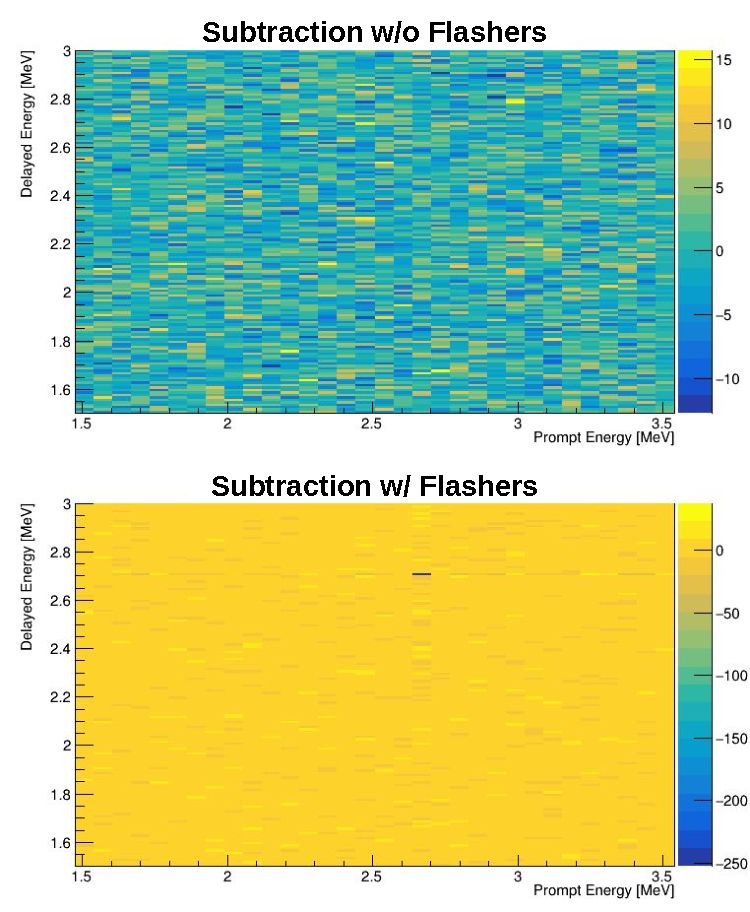
\includegraphics[width=0.73\textwidth]{ch_simulation/flasher_prompt_delayed}
    \caption[Simulated residual flashers impact]{
        Accidentals-subtracted prompt vs. delayed energy for simulated data samples
        including only Single events (top) or Single and Flasher events (bottom).
        The Singles-only histogram correctly shows 0 events remaining
        after subtracting the accidental background.
        In the with-Flashers histogram,
        the single energy bin containing (\SI{2.7}{\MeV}, \SI{2.7}{\MeV})
        (the energy of the simulated Flasher events)
        has a negative bin content,
        validating that the Flasher events
        will contaminate the synthetic accidental background,
        form Flasher-Flasher pairs, and cause a distortion to the subtracted spectrum.
        Figure taken from \cite{flasher_sim}.
    }
    \label{fig:sim_flasher_prompt_delayed}
\end{figure}

\section{Fake experiment simulation}
\label{sec:lbnl_toymc}

An independent simulation was implemented
to generate spectra of reconstructed prompt energy for each AD,
under assumptions of a wide variety of systematic uncertainties,
backgrounds, and reactor parameters.
Since the simulation output was designed to include all the necessary inputs
to the \thetaot{} fitter,
the outputs were known as ``fake experiments;''
the simulation itself will be referred to as the Fake Experiment Simulation (FES).
This simulation was originally \cite{lbnl_toymc,p12e_fitter,p14a_fitter} designed to generate covariance matrices for
and validate the performance of
one of the fitter programs for the nGd analysis
(Method A of \cite{ngd2016}).
It was used essentially unmodified to validate the fitter for this (nH) analysis
(\cref{ch:analysis}).

The FES received as input predicted \nuebar{} flux and spectrum data
which were computed \cite{christine_reactor} based on data from the reactor operator
and the models by Huber \cite{reactor_huber}
and Mueller \emph{et al.} \cite{reactor_mueller} (see also \cref{sec:reactor}).
For each reactor-AD pair, the spectra were evolved
based on the configured oscillation parameters
and suppressed by $\nicefrac{1}{L^2}$ due to isotropic emission.
The true \nuebar{} spectrum for IBD interactions was computed
based on the IBD cross section \cite{ibd_xsec,ibd_xsec_note},
number of target protons, and the projected reactor flux.
The detection efficiencies and muon and multiplicity veto efficiencies
were also applied.
A model for the detector response was applied to the true interaction energy
to account for the conversion to positron energy,
energy losses in the IAV,
energy nonlinearities in the scintillator and electronics,
and the energy resolution.
The final simulated energies could be scaled by a fixed factor
to account for the relative energy scale uncertainty.
All of the quantities just mentioned could be configured
to be either known or uncertain, in which case
the relevant values in the simulation would be
adjusted by a configurable random amount
to simulate a systematic uncertainty.
Predicted rates and spectra for background events
were added after the IBD prompt spectra were fully generated.
The backgrounds could be randomly fluctuated to account for
uncertainties in their rates and spectra.
Lastly, the number of events in each bin of prompt reconstructed energy
could optionally be fluctuated to account for statistical uncertainty
before being output as the results of the simulation.
\Cref{fig:lbnl_toymc_flowchart} shows the above steps as a flowchart.

\begin{figure}
    \centering
    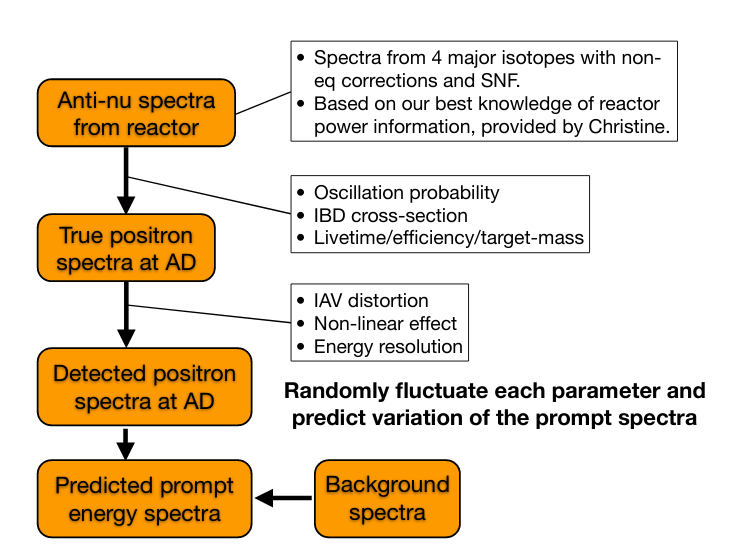
\includegraphics[width=0.6\textwidth]{ch_simulation/lbnl_toymc_flowchart}
    \caption[Flowchart of data set toy Monte Carlo]{
        Steps to simulate the prompt reconstructed spectra
        at each AD.
        Figure taken from \cite{lbnl_toymc}.
    }
    \label{fig:lbnl_toymc_flowchart}
\end{figure}

\subsection{Study of fitter accuracy}
\label{subsec:fitter_validation}

The fitter developed in \cref{ch:analysis} was validated
using simulated data sets with known values of \thetaot{}.
The degree to which the fitter could extract
the ``correct'' (input) value of \thetaot{}
was a measure of its accuracy
and helped verify that there were no major software bugs
which could have caused an incorrect measurement of \thetaot{}.
The nH and nGd analyses were similar enough
that the same fitter software could be used for both analyses
simply by adjusting the values for uncertainties, efficiencies,
target masses and backgrounds
(and, of course, using the corresponding prompt-energy spectra).
Thus the data set toy Monte Carlo was used without modification
to generate simulated nGd data sets,
and the fitter was validated without relying on
any aspects of the nH analysis.

Data sets were generated under each test configuration
for 36 pairs of (\thetaot{}, \dmee{}) mixing parameters.
(\dmee{} was used only as an input value,
and was converted to $\Delta m^2_{32}$ internally.)
The input values of $\sin^22\thetaot{}$ ranged from 0.065 to 0.09
in steps of 0.005;
those of \dmee{} ranged from
\SI{2.3e-3}{\eV\squared} to \SI{2.7e-3}{\eV\squared}
in steps of \SI{0.08e-3}{\eV\squared}.

The fitter was tested against data sets
that were configured to have no statistical or systematic fluctuations
in order to verify the precise performance
of the prediction algorithm and minimizer.
Since these simulations were fully deterministic,
only one data set was generated for each of the 36 parameter combinations.
The fitter was also tested against data sets
that included fluctuations, both statistical and systematic in nature.
To thoroughly exercise the fitter's functionality
for each configuration,
1000 data sets were generated
for each of the 36 parameter combinations,
for a total of \num{36000} simulated data sets per configuration.
The full listing of configurations tested
is shown in \cref{tab:validation_configs}.
For the final validation, with all systematic and statistical fluctuations
and all pull parameters enabled,
a smaller sample of 190 data sets for each of 9 parameter combinations
(total of \num{1710} data sets)
was used since the full fitter with all pull parameters
took substantially longer to run than it did with any subset of pull parameters.

\ctable[
cap = Fitter validation simulation configurations,
caption = {
    Simulation configurations for validating the fitter performance.
},
label = tab:validation_configs,
pos = ht
]{ll}{
    \tnote[a]{
        Composite nonlinearity functions were generated
        from 5 independent models
        each contributing in random proportions to the composite.
    }
    \tnote[b]{
        Uncertainties from non-equilibrium isotopes,
        spent nuclear fuel contribution,
        correlated and uncorrelated model uncertainties.
    }
}{\FL
    & Fluctuation RMS \ML
    Statistics (EH3) & Poisson \NN
    Statistics (EH1 \& EH2) & Poisson \NN
    Detection efficiency & \SI{0.3}{\percent} \NN
    Relative energy scale & \SI{0.2}{\percent} \NN
    Absolute energy scale & $\lesssim\SI{2}{\percent}$\tmark[a] \NN
    Energy resolution & $\SI{0.2}{\percent}/\sqrt{E/\si{\MeV}}$ \NN
    Reactor power & \SI{0.8}{\percent} \NN
    Reactor \nuebar{} spectrum & \SI{5}{\percent} fission fraction, etc.\tmark[b] \NN
    Input mixing parameters & Values from \cite{pdg} \NN
    Accidental background & \parbox[t]{5cm}{
        \SI{0.13}{\percent} (EH1), \SI{0.17}{\percent} (EH2) \\
        \SI{0.42}{\percent} (EH3)
    } \NN
    \li{}/\he{} background & \parbox[t]{5cm}{
        \SI{27}{\percent} (EH1), \SI{29}{\percent} (EH2) \\
        \SI{33}{\percent} (EH3)
    } \NN
    Fast-neutron background & \SI{10}{\percent} (EH1 \& EH2), \SI{17}{\percent} (EH3) \NN
    \amc{} background & \SI{50}{\percent} \NN
    \bottomrule
}

\begin{figure}
    \centering
    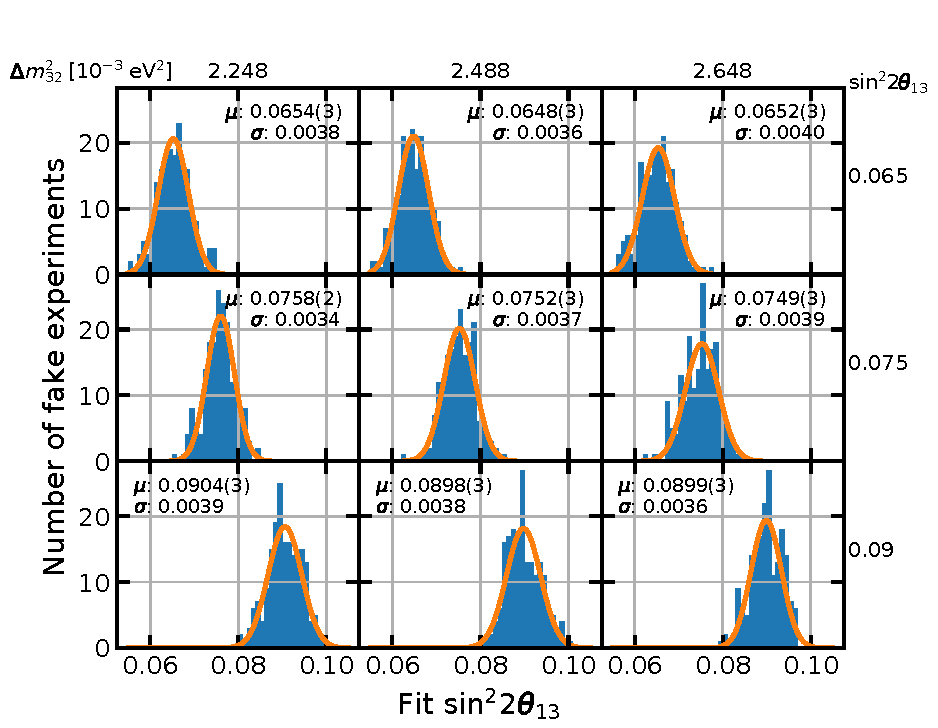
\includegraphics{ch_simulation/validation_final_sin2_annotated}
    \caption[Fitter validation results]{
        Distribution of the extracted $\sin^22\thetaot{}$
        for 9 combinations of \thetaot{} and $\Delta m^2_{32}${},
        with 190 fake experiments per combination,
        with all simulated systematics and all fitter pull parameters enabled.
        Each row shares a true (input) $\sin^22\thetaot{}$,
        and each column shares a true $\Delta m^2_{32}$.
        The listed $\mu$ and $\sigma$ are the sample mean and standard deviation,
        respectively, for each 190-experiment sample.
        The standard error of the mean is indicated in parentheses
        as the uncertainty in the last digit.
        The orange curves are the best-fit Gaussian distributions
        to each sample.
    }
    \label{fig:final_validation}
\end{figure}

The distribution of extracted $\sin^22\thetaot$ values from the final validation
is shown in \cref{fig:final_validation}.
For 6 of the 9 parameter combinations (\SI{66}{\percent}),
the mean extracted $\sin^22\thetaot$
was within $\pm1$ standard error of the ``true'' (simulation input) $\sin^22\thetaot$,
demonstrating the statistical consistency of the fitter and simulation infrastructure.
A second consistency check was the distribution of minimum $\chi^2$ values
from the fitter,
which should follow the $\chi^2$ distribution with 3 degrees of freedom
(see \cref{subsec:fitter_specification}).
When all pull parameters were disabled (that is, fixed at 0), the extracted $\chi^2$ values
did indeed follow the theoretical predicted distribution.
However, as shown in \cref{fig:validation_chi2},
when all nuisance parameters were enabled as parameters of the fit,
the $\chi^2$ values decreased to lower values than the prediction.
This discrepancy was traced to the use of the nuisance parameters
modeling the AD-to-AD variation in detection efficiency;
when these parameters were disabled but all others were enabled,
the extracted $\chi^2$ values still matched the prediction for 3 degrees of freedom.
An explanation was identified for this effect.
Each nuisance parameter controls the efficiency for a single AD,
modeled as a multiplicative factor of the final predicted number of events at an AD.
Thus after the prediction based on the near-hall observations is made,
any difference between the prediction and observation at a far-hall AD
can be reduced by updating the efficiency nuisance parameter for that AD.
Even with the constraint on the value of the nuisance parameter,
an improvement to the overall $\chi^2$
beyond the usual statistical expectation
can usually be obtained by this mechanism.

In any event, the impact of the nuisance parameters
on the extracted $\sin^22\thetaot{}$ was minimal.
Over the 1710 fake experiments used for final validation, the maximum discrepancy in $\sin^22\thetaot{}$
between a fit with no pull parameters and one with all enabled
was \SI{0.08}{\percent}.

\begin{figure}
    \centering
    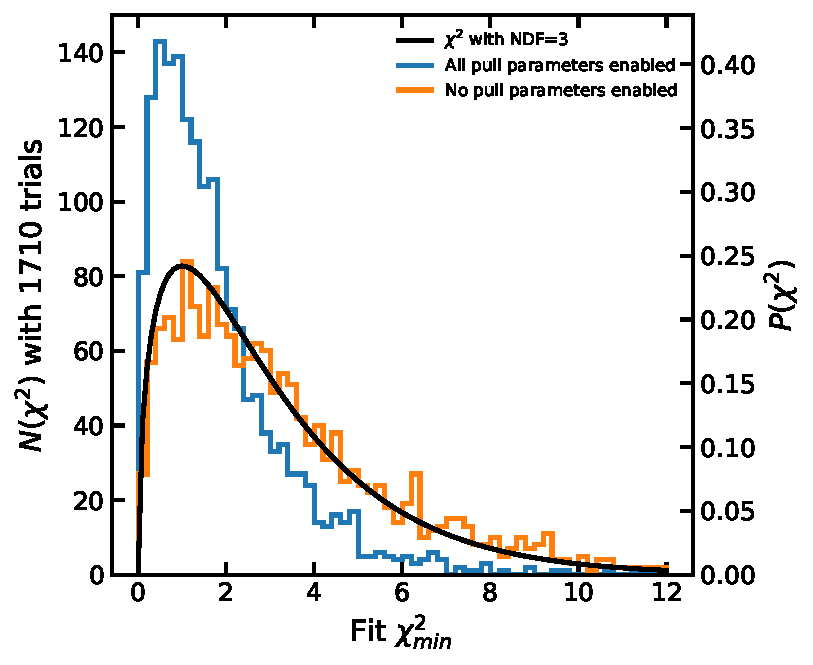
\includegraphics{ch_simulation/validation_chi2_dist}
    \caption[Fitter validation $\chi^2$ distribution]{
        Distribution of the fit minimum $\chi^2$
        for the \num{1710} fake experiments
        simulated with all systematics.
        The blue histogram shows the results with all pull parameters enabled;
        it has a lower mean than would be expected from the 3 degrees of freedom.
        The orange histogram shows that with all pull parameters disabled,
        the distribution of the minimum $\chi^2$ matches the theoretical prediction
        for 3 degrees of freedom (black curve).
        The scale on the right-hand vertical axis gives the probability density
        for the theoretical prediction.
    }
    \label{fig:validation_chi2}
\end{figure}

